\documentclass[10pt,letterpaper,fleqn]{article}

\usepackage[utf8]{inputenc}
\usepackage[spanish,es-nodecimaldot]{babel}
\usepackage{amsmath}
\usepackage{amssymb}
\usepackage{multicol}
\usepackage{graphicx}
\usepackage{mdwlist}

\usepackage[dvipsnames]{xcolor}
\usepackage[most]{tcolorbox}

\usepackage{tabu}

\usepackage{mathtools}

\usepackage[top=1in, bottom=1in, left=1in, right=1in]{geometry}


\begin{document}

\begin{titlepage}
    \centering

    {\scshape\LARGE Universidad Nacional Autónoma de México \par}

    \vspace{1cm}
    {\scshape\Large Facultad de Ciencias\par}
    \vspace{1.5cm}

    \begin{center}
        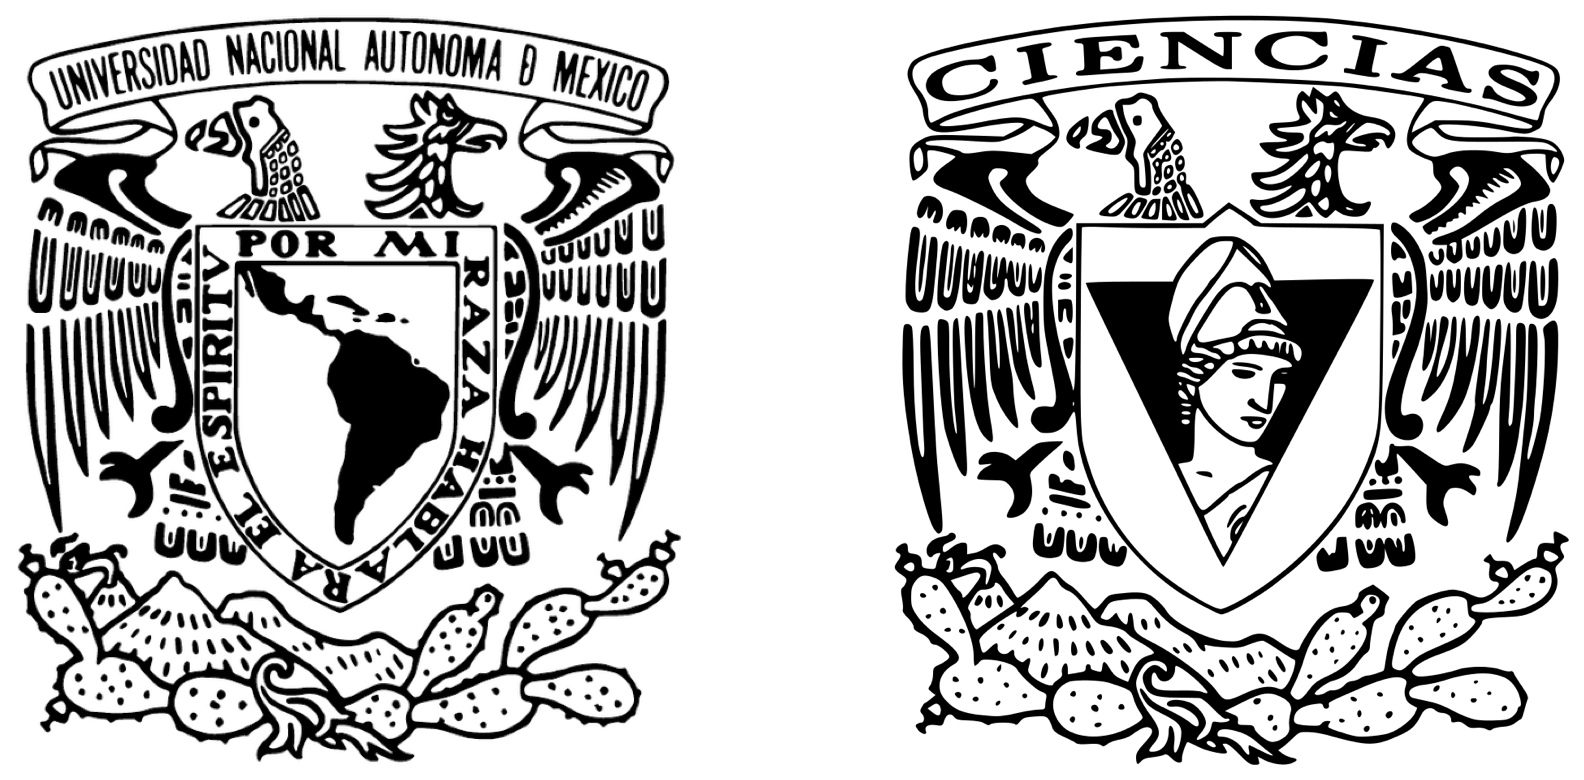
\includegraphics[scale=.1]{assets/img/logo.png}
    \end{center}

    \vspace{.8 cm}

    {\LARGE Tarea 1: \par}
    {\huge\bfseries Ejercicios \par}

    \vspace{0.5cm}
    \large{\itshape{Luis Erick Montes Garcia}} \small{ - 419004547}\\
    \large{\itshape{Hele Michelle Salazar Zaragoza}} \small{ - 316068895}


    \vfill

    Trabajo presentado como parte del curso de
    \textbf{Matematicas Aplicadas para las Ciencias II}
    impartido por el profesor \textbf{Juan Carlos Balleza}. \par
    \vspace{0.1cm}
    {\large Entrega 1 de Marzo 2019 \par}
    \footnotesize{\textbf{Link al código fuente:} git@github.com:lemg98/Matematicas-Aplicadas-II.git}
\end{titlepage}

    \begin{enumerate}
        %Ejercicio 1.
        \item Sea la función vectorial $r(\overrightarrow{t}) = \left(\frac{t}{t+1},\frac{1}{t}\right)$. A continuación responda lo siguiente:
        \begin{itemize}
        	\item Calcule el siguiente límite: $$ lim_{t\rightarrow -1}r(\overrightarrow{t})$$
        	\textbf{Solución:} Observamos que al acercarnos a -1 por la izquierda $t+1$ se hace pequeño negativamente, por tanto 
        	$\frac{t}{t+1}$ tiende a infinito de manera negativa, análogamente sucede cuando nos acercamos a -1 por la derecha, este
        	tiende a infinito positivamente. Por tanto no existe el límite en ese punto


        	\item Calcule el siguiente límite: $$ lim_{t\rightarrow 0}r(\overrightarrow{t})$$
        	\textbf{Solución:} Sucede de la misma manera con este límite. Si tiende a 0 por la izquierda $\frac{1}{t}$ tiende a infinito
        	negativamente. Análogamente cuando tiende por la derecha esto tiende a infinito.

        	\item ¿Para qué valores de $t$ es discontinua la función $r(\overrightarrow{t})$? Explique su resultado.\\
        	\textbf{Solución:} Como ya mencionamos en los dos puntos anteriores no existe el límite, en los demás la función
        	es continua. Por tanto en los puntos 0 y -1 la función es discontinua.

        	\item Obtenga y dibuje los vectores velocidad y aceleración, en el punto donde $t = -\frac{1}{2}$.\\
        	\textbf{Solución:} Encontramos la primera derivada y valuamos
        	\begin{equation*}
        	\begin{split}
        		r'(\overrightarrow{t}) &= \left(\left(\frac{t}{t+1}\right)',(\frac{1}{t})'\right) \\
        							   &= \left(\frac{1(t+1) - 1(t)}{(t+1)^2},-\frac{1}{t^2}\right) \\
        							   &= \left(\frac{1}{(t+1)^2},-\frac{1}{t^2}\right) \\
				r'(\overrightarrow{-\frac{1}{2}}) &= \left(\frac{1}{(-\frac{1}{2}+1)^2},-\frac{1}{(\frac{1}{2})^2}\right) \\        							   &= \left(4,-4\right)
        	\end{split}
        	\end{equation*}

        	Encontramos ahora la segunda derivada y valuamos
        	\begin{equation*}
        	\begin{split}
        		r''(\overrightarrow{t}) &= \left(\left(\frac{1}{(t+1)^2}\right)',-\left(\frac{1}{t^2}\right)'\right) \\
        								&= \left(-\frac{2(t+1)}{(t+1)^4},-\left(\frac{1}{t^2}\right)'\right) \\
        								&= \left(-\frac{2}{(t+1)^3},\frac{1}{t^4}\right) \\
        		r''(\overrightarrow{-\frac{1}{2}}) &= \left(-\frac{2}{(-\frac{1}{2}+1)^3},\frac{1}{(-\frac{1}{2})^4}\right) \\
        								&= \left(-\frac{2}{(-\frac{1}{2}+1)^3},\frac{1}{(-\frac{1}{2})^4}\right) \\
        								&= \left(-16,16\right) \\
        	\end{split}
        	\end{equation*}


        \end{itemize}

        %Ejercicio 2.
        \item Sea la función vectorial $r (\overrightarrow{t}) = (4cos({t \over 2}),4sin({t \over 2}))$, donde $t \in [0,2\pi]$. A continuación responda lo siguiente:
        %Incisos del ejercicio 2.
        \begin{enumerate}
            %Inciso a
            \item Calcule los vectores de velocidad y aceleración.
            \\ Obtenemos la derivada de la función  $r (\overrightarrow{t})$ para obtener la {\bf velocidad}: 
            \begin{center}
                $r'(\overrightarrow{t}) = (-2sin({t \over 2}),2cos({t \over 2}))$ 
            \end{center}

            Obtenemos la derivada de la función $r'(\overrightarrow{t})$ para obtener la {\bf aceleración}:
            \begin{center}
                $r''(\overrightarrow{t}) = (-cos({t \over 2}),-sin({t \over 2}))$ \\
                \begin{tabular}{|c|c|c|} \hline 
                    t & velocidad & aceleración \\ \hline
                    $0$ & $(0,2) $ & $(-1,0)$  \\ \hline
                    $2\pi$ & $(-0.109,1.99)$ & $(-0.99,-0.054)$  \\ \hline
                \end{tabular}
            \end{center}

            %Inciso b
            \item Grafique la función vectorial, en el intervalo de $t$ indicado.
            \begin{center}
                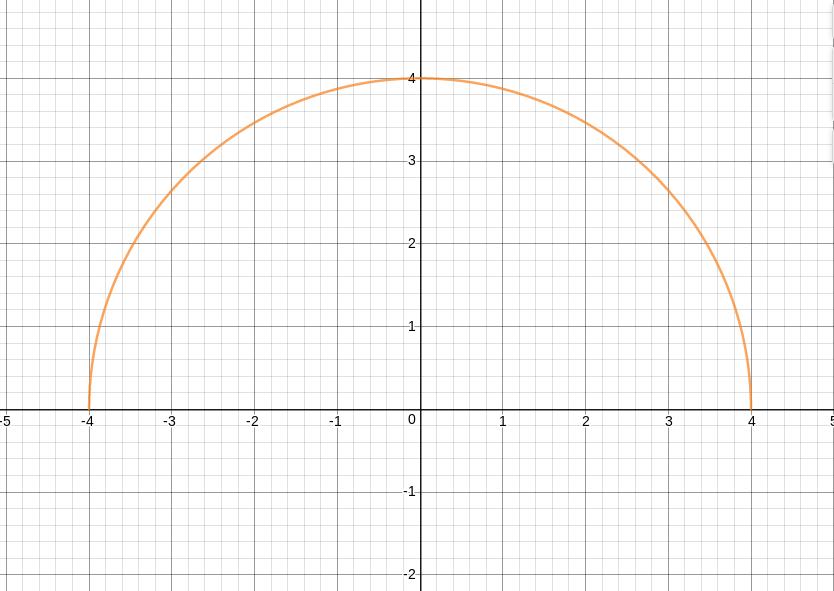
\includegraphics[scale=.3]{assets/img/ejercicio2(b).png}
            \end{center}
            %Inciso c
            \item En la gráfica de la función vectorial (inciso anterior), agregue los vectores de velocidad y aceleración en el instante $t = \pi$ 
            \begin{center}
                \begin{tabular}{|c|c|c|} \hline 
                    t & velocidad & aceleración \\ \hline
                    $\pi$ & $(-0.054,1.99) $ & $(-0.99,-0.02)$  \\ \hline
                \end{tabular}
                \\
                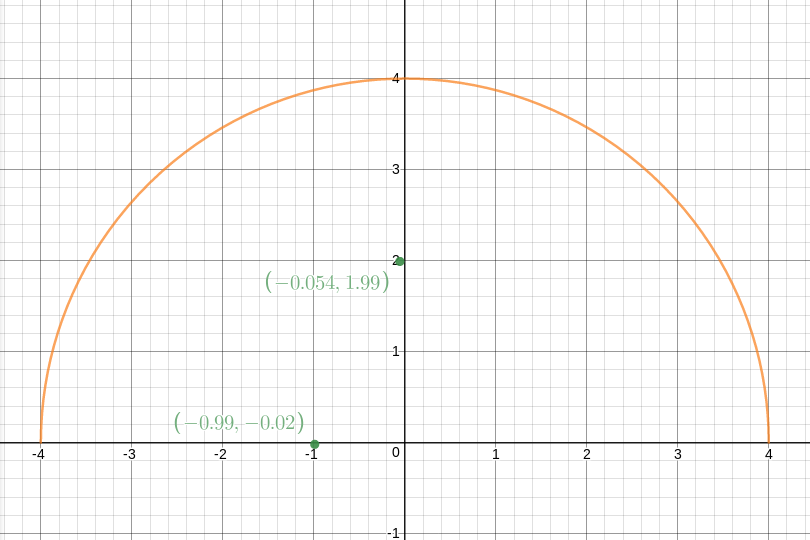
\includegraphics[scale=.3]{assets/img/ejercicio2(c).png}
            \end{center}

            %Inciso d
            \item Obtenga el ángulo entre los vectores velocidad y aceleración.
            \\ Decimos que el vector de velocidad es el vector $\overrightarrow{a}$ y que el vector de aceleración es $\overrightarrow{b}$. Para obtener el ángulo $\theta$ formamos un triángulo, siendo $\overrightarrow{a}-\overrightarrow{b}$ el lado opuesto al ángulo.
            \\ Aplicando ley de cosenos, tenemos que: \\
            $||\overrightarrow{a}-\overrightarrow{b}||^2=||\overrightarrow{a}||^2 + ||\overrightarrow{b}||^2-2||\overrightarrow{a}|| ||\overrightarrow{b}|| cos \theta $ \\
            Sustituímos: \\
        \end{enumerate}


        %Ejercicio 3.
        \item Sea la función vectorial $r(\overrightarrow{t})=(t^2, 2t-1, t^3)$. Proporcione las ecuaciones paramétricas de
        la recta que es tangente a la curva, en el punto $t_0=2$.\\
        \textbf{Solución:} Obtenemos $r(2)= (2^2,2(2) -1 , 2^3)=(4, 3, 8)$. Observamos $$r' = (2t,2,3t^2)$$, obtenemos
        $r'(2) = (2(2),2,3(2)^2) = (4,2,12)$, este es el vector de dirección. Por tanto las ecuaciones paramétricas son
        \begin{equation*}
        \begin{split}
        	x &= 4t + 4 \\
        	y &= 2t + 3 \\
        	z &= 12t + 8
        \end{split}
        \end{equation*} 

        %Ejercicio 4.
        \item Proporcione la función vectorial $r(\overrightarrow{t})$, tal que cumpla las siguientes condiciones:
        %Incisos del Ejercicio 4.
        \begin{enumerate}
            %Inciso a
            \item $a(t)=(-1,-1,-1)$
            %Inciso b
            \item $v(0)=(0,0,0)$
            %Inciso c
            \item $r(0)=(10,10,10)$
        \end{enumerate}
(
        %Ejercicio 5.
        \item En el instante $t = 0$, una partícula se encuentra en el punto $A(1,2,3)$. Viaja siguiendo una línea recta
        hasta el punto (4,1,4) y tiene una rapidez de 2(en el punto $A$) y aceleración constante $a(t) = 3i - j + k$.
        Proporcione la ecuación del vector de posición $r(t)$ en el instante $t$.

        %Ejercicio 6.
        \item Considere la función vectorial $r(\overrightarrow{t})= ([cos t]^3,[sin t]^3)$. Responda lo siguiente:
        %Incisos del Ejercicio 6.
        \begin{enumerate}
            %Inciso a
            \item Obtenga el vector tangente unitario a la curva.
            %Inciso b
            \item Calcule la longitud de la curva para $t \in [0,{\pi \over 2}]$
        \end{enumerate}

        %Ejercicio 7.
        \item

        %Ejercicio 8.
        \item Obtenga la ecuación del círculo osculador para la función $y=sin x$ en el punto de coordenadas $({\pi \over 2},1)$. Proponga $r(\overrightarrow{t})$ a partir de la "parametrización trivial" de la función. Calcule lo siguiente: 
        %Incisos del Ejercicio 8.
        \begin{enumerate}
            \item $(\overrightarrow{T})$, $(\overrightarrow{N})$ y $k$.
        \end{enumerate}
        Haga una gráfica con la siguiente información:
        \begin{enumerate}
            \item La función $y=sin x$
            \item El círculo osculador y además localizar el punto de coordenadas $({\pi \over 2},1)$
            \item Los vectores $(\overrightarrow{T})$, $(\overrightarrow{N})$.
        \end{enumerate}

        %Ejercicio 9
        \item 


    \end{enumerate}





\end{document}